Pipeline é uma técnica bem antiga e bastante conhecida por ser empregada na
linha de produção industrial. A ideia por trás dessa técnica é bastante simples.
Um processo passa por vários estágios da linha de montagem, subdividindo em
tarefas menores, e essa linha de montagem é continuamente alimentada de novos
processos. Em cada estágio uma parte de um processo é finalizado e passado para
o próximo estágio. Quando é chegado no ultimo estágio, cada subprocesso
finalizado é reunido e então finalmente finalizado
completamente~\cite{Bhujade95}. Um bom exemplo da aplicação dessa técnica é na
industria automobilística onde são construídos diversos carros simultaneamente.
A Figura~\ref{fig:carro} mostra a ilustração da aplicação do pipeline na linha
de montagem de um carro.

\begin{figure}[!h]
	\centering
	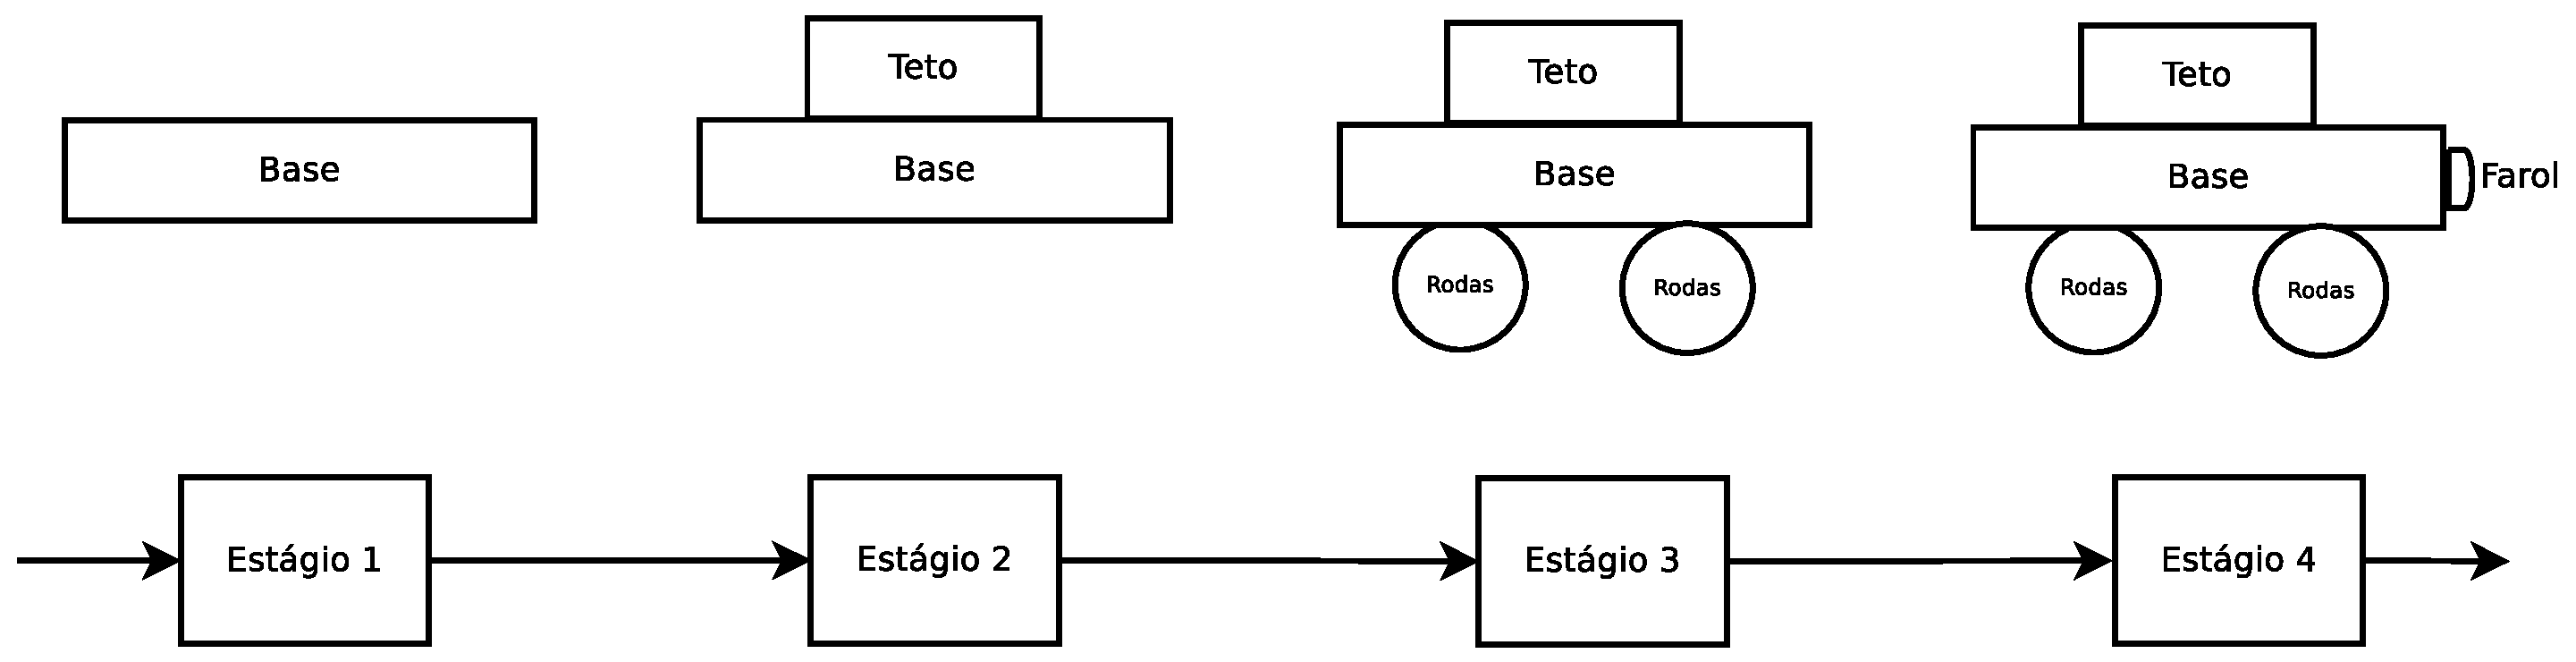
\includegraphics[width=0.95\linewidth]{figs/carro}
	\caption{Processo de uma linha de montagem da industria automobilística.}
	\label{fig:carro}
\end{figure}

Na computação essa técnica foi também incorporada para o desenvolvimento de
programas. Com a grande variedade de processadores multicore, houve a
necessidade de aproveitar ao máximo o poder de processamento de cada núcleo do
processador. A execução de tarefas sequenciais não é a melhor forma de obter
alto desempenho de processamento. Nesse sentido, o pipelining se torna uma
técnica alternativa para aumentar o desempenho de tarefas sequenciais de
\textit{software}.

Ao utilizar a técnica de pipelining, um processo que normalmente seria
executado de forma sequencial é dividido em estágios distintos que podem ser
executados em um modelo de linha de montagem semelhante ao exemplo mostrado
anteriormente, onde dada núcleo do processador fica encarregado de executar uma
subtarefa. 

Dessa forma, o pipelining melhora o desempenho, pois a subdivisão de uma tarefa
em tarefas menores executadas cada uma por um certo processador é mais rápido
para ser finalizada que se cada uma das subtarefas fossem executadas apenas por
um único processador.

É importante ressaltar que para haver uma melhora significativa no desempenho, é
sempre recomendável manter o balanceamento das subtarefas. A
Figura~\ref{fig:bal} mostra a questão do balanceamento.

\begin{figure}[!h]
	\centering
	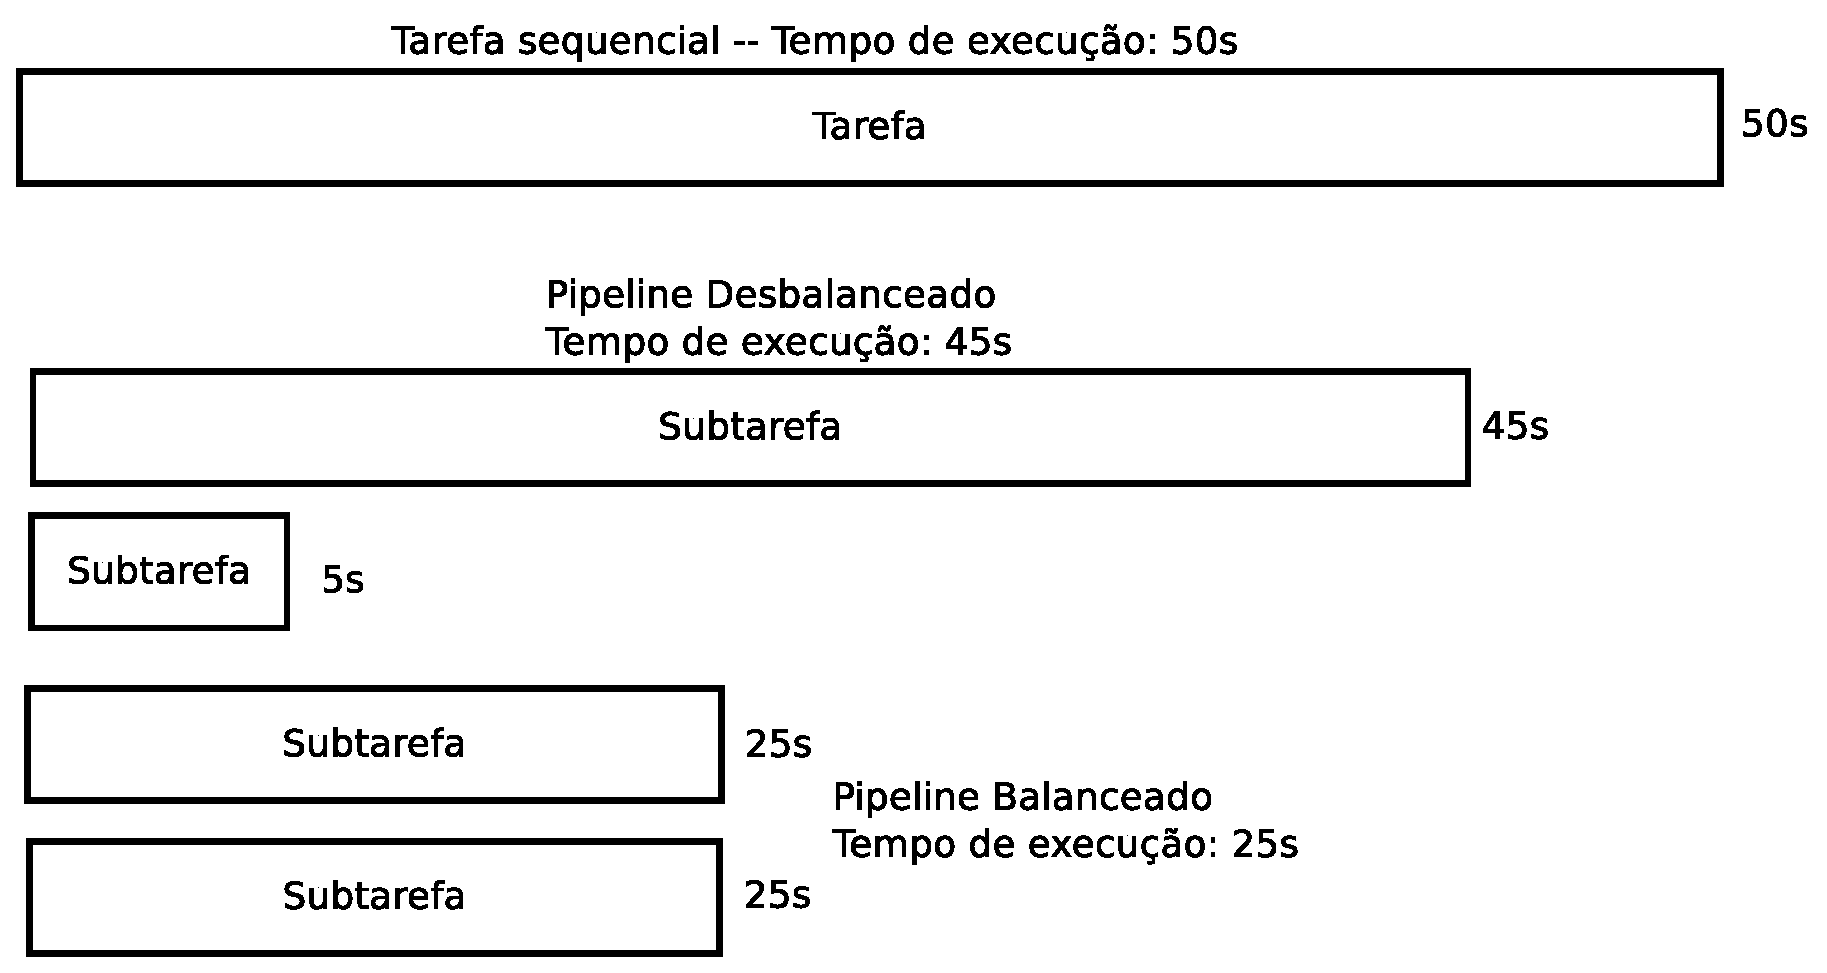
\includegraphics[width=0.95\linewidth]{figs/pipe}
	\caption{Balanceamento de subtarefas.}
	\label{fig:bal}
\end{figure}

O primeiro caso da Figura~\ref{fig:bal} mostra o tempo de execução de uma tarefa
sequencial. Aplicando técnica de pipelining sem levar em conta a questão do
balanceamento, como mostra o segundo caso, o tempo para executar tarefa reduz
pouco se levarmos em conta o tempo da tarefa sequencial. Contudo, se o pipeling
for aplicado com as subtarefas balanceados, o desempenho de execução melhora
consideravelmente, sendo justificável a aplicação dessa técnica para este caso,
visto que o tempo de execução é reduzido pela metade.
